\chapter{TINJAUAN PUSTAKA}


% Ubah bagian-bagian berikut dengan isi dari tinjauan pustaka

\section{Hasil Penelitian/Perancangan Terdahulu}

\subsection{\textit{A Transformer-based Framework for Multivariate Time Series Representation Learning}}
 Penelitian ini mengkaji tentang arsitektur Transformer untuk representasi data time series multivarian dengan kerangka yang baru.Model yang digunakan dalam model ini menggunakan strategi masking,di mana sebagian data time series disembunyikan selama pelatihan. Model kemudian dilatih untuk merekonstruksi bagian yang disembunyikan, sehingga meningkatkan kemampuannya untuk menangkap pola dan generalisasi ke berbagai tugas time series. Untuk menangkap informasi temporal dalam data, penulis mengganti encoding posisi sinusoidal standar dengan encoding posisi yang dapat dipelajari, yang terbukti lebih efektif dalam time series. Model ini difokuskan pada efeisiensi komputasi, sehingga arsitektur hanya menggunakan encoder transformer tanpa decoder, membuatnya lebih ringan dan efisien untuk data time series multivarian.
 
\subsection{\textit{Are Transformers Effective for Time Series Forecasting?}}
 Penelitian ini bertujuan untuk mengevaluasi efektivitas model Transformer dalam tugas peramalan deret waktu (time series forecasting). Para peneliti ingin memahami apakah arsitektur Transformer, yang terkenal dalam pemrosesan bahasa alami, dapat bersaing dengan atau bahkan melampaui model yang telah ada dalam domain peramalan deret waktu.Disimpulkan bahwa Transformer memiliki potensi yang besar untuk tugas peramalan deret waktu, terutama pada skenario yang melibatkan ketergantungan jangka panjang. Namun, penerapannya harus mempertimbangkan sumber daya komputasi yang tersedia serta kebutuhan spesifik dari tugas peramalan. Dengan adaptasi yang tepat, Transformer dapat menjadi alat yang sangat kuat untuk memodelkan deret waktu.

\subsection{\textit{Transformers in Time Series: A Survey}}
Penelitian ini bertujuan untuk menyajikan tinjauan komprehensif tentang penerapan dan perkembangan model Transformer dalam domain deret waktu. Dengan semakin meluasnya penggunaan Transformer di berbagai bidang, penelitian ini mengeksplorasi potensi, tantangan, dan inovasi terkini dalam penerapan model ini untuk berbagai tugas peramalan, deteksi anomali, klasifikasi, dan segmentasi deret waktu. Transformer menawarkan pendekatan yang menjanjikan untuk berbagai tugas deret waktu. Namun, implementasinya masih menghadapi tantangan dalam hal efisiensi dan kebutuhan sumber daya. Dengan inovasi yang berkelanjutan, Transformer diproyeksikan akan menjadi pondasi penting dalam analisis deret waktu yang kompleks dan berskala besar.

\section{Teori/Konsep Dasar}

\subsection{Pasar modal}

% Contoh penggunaan referensi dari pustaka
Pasar modal adalah tempat di mana sekuritas seperti saham, obligasi, dan instrumen keuangan lainnya diperdagangkan. Pasar modal memungkinkan perusahaan untuk mendapatkan dana dengan menawarkan saham atau obligasi kepada publik. Selain itu, investor dapat membeli dan menjual sekuritas tersebut untuk memperoleh keuntungan.Pasar modal memiliki peran penting dalam ekonomi karena menyediakan likuiditas bagi investor dan membantu perusahaan untuk mendapatkan dana yang dibutuhkan untuk ekspansi\autocite{mishkin2018financial}. Beberapa instrumen yang diperdagangkan di pasar modal adalah saham, obligasi, dan derivatif.Harga di pasar modal dipengaruhi oleh berbagai faktor, termasuk kondisi ekonomi, suku bunga, inflasi, kebijakan pemerintah, dan kondisi pasar global.
\begin{figure} [H] \centering
  % Nama dari file gambar yang diinputkan
  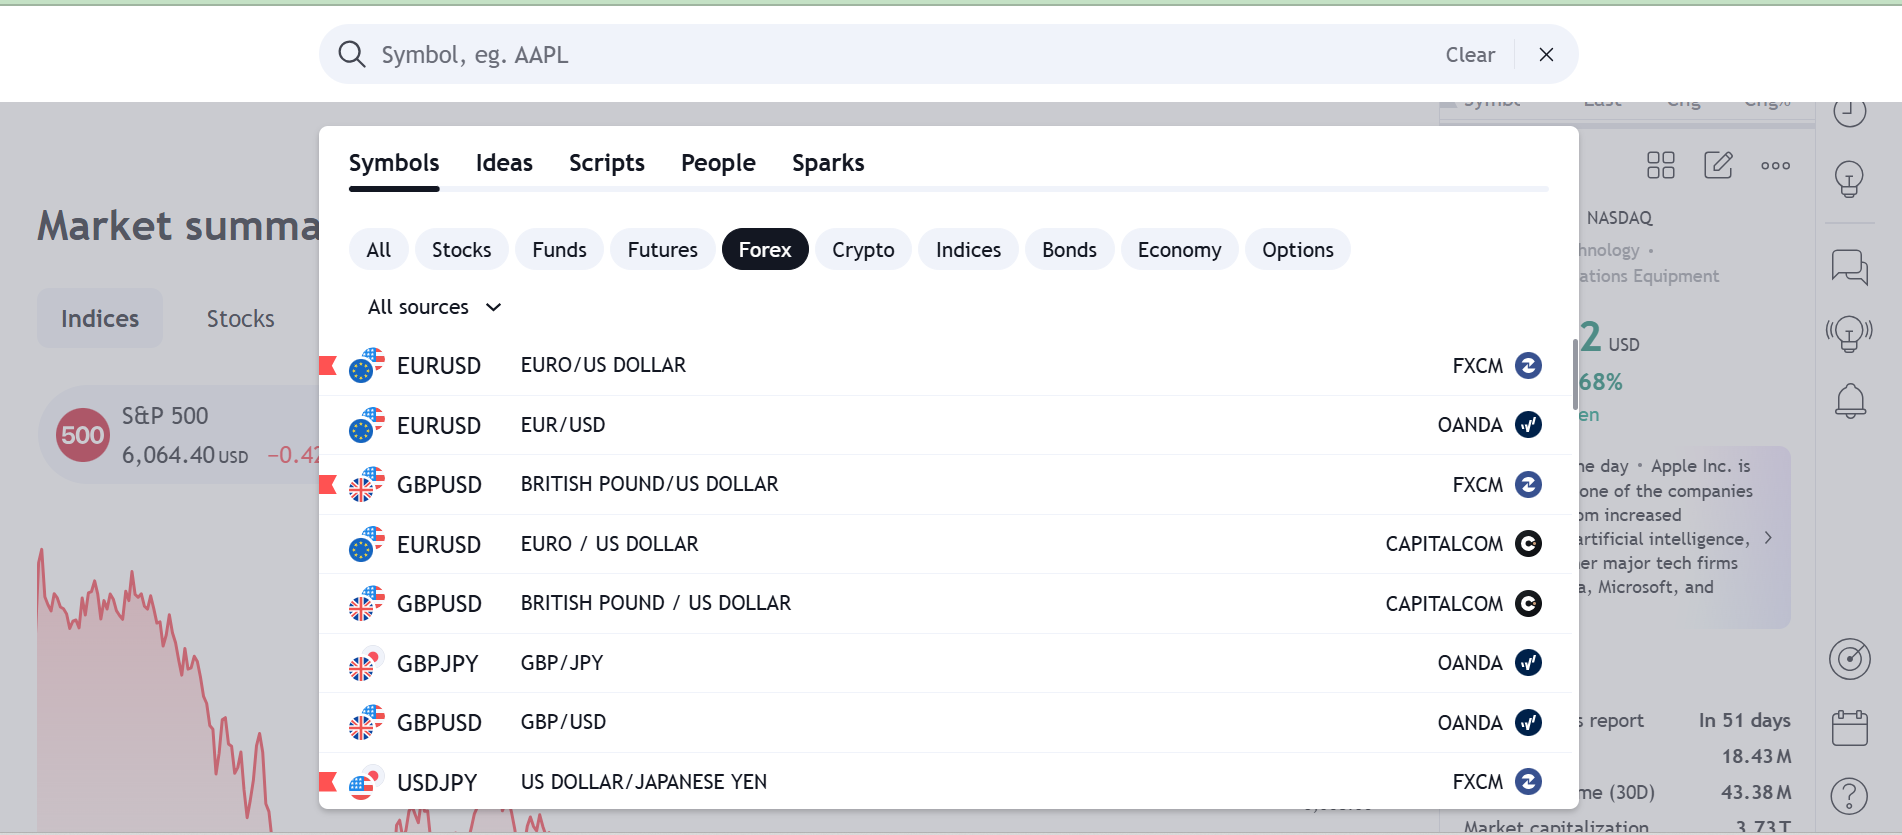
\includegraphics[scale=0.4]{gambar/gambarpasarmodalbeneran.png} 
    \caption{Overview Pasar Modal}
    \label{fig:label_gambar}
\end{figure}

\begin{figure} [H] \centering
  % Nama dari file gambar yang diinputkan
  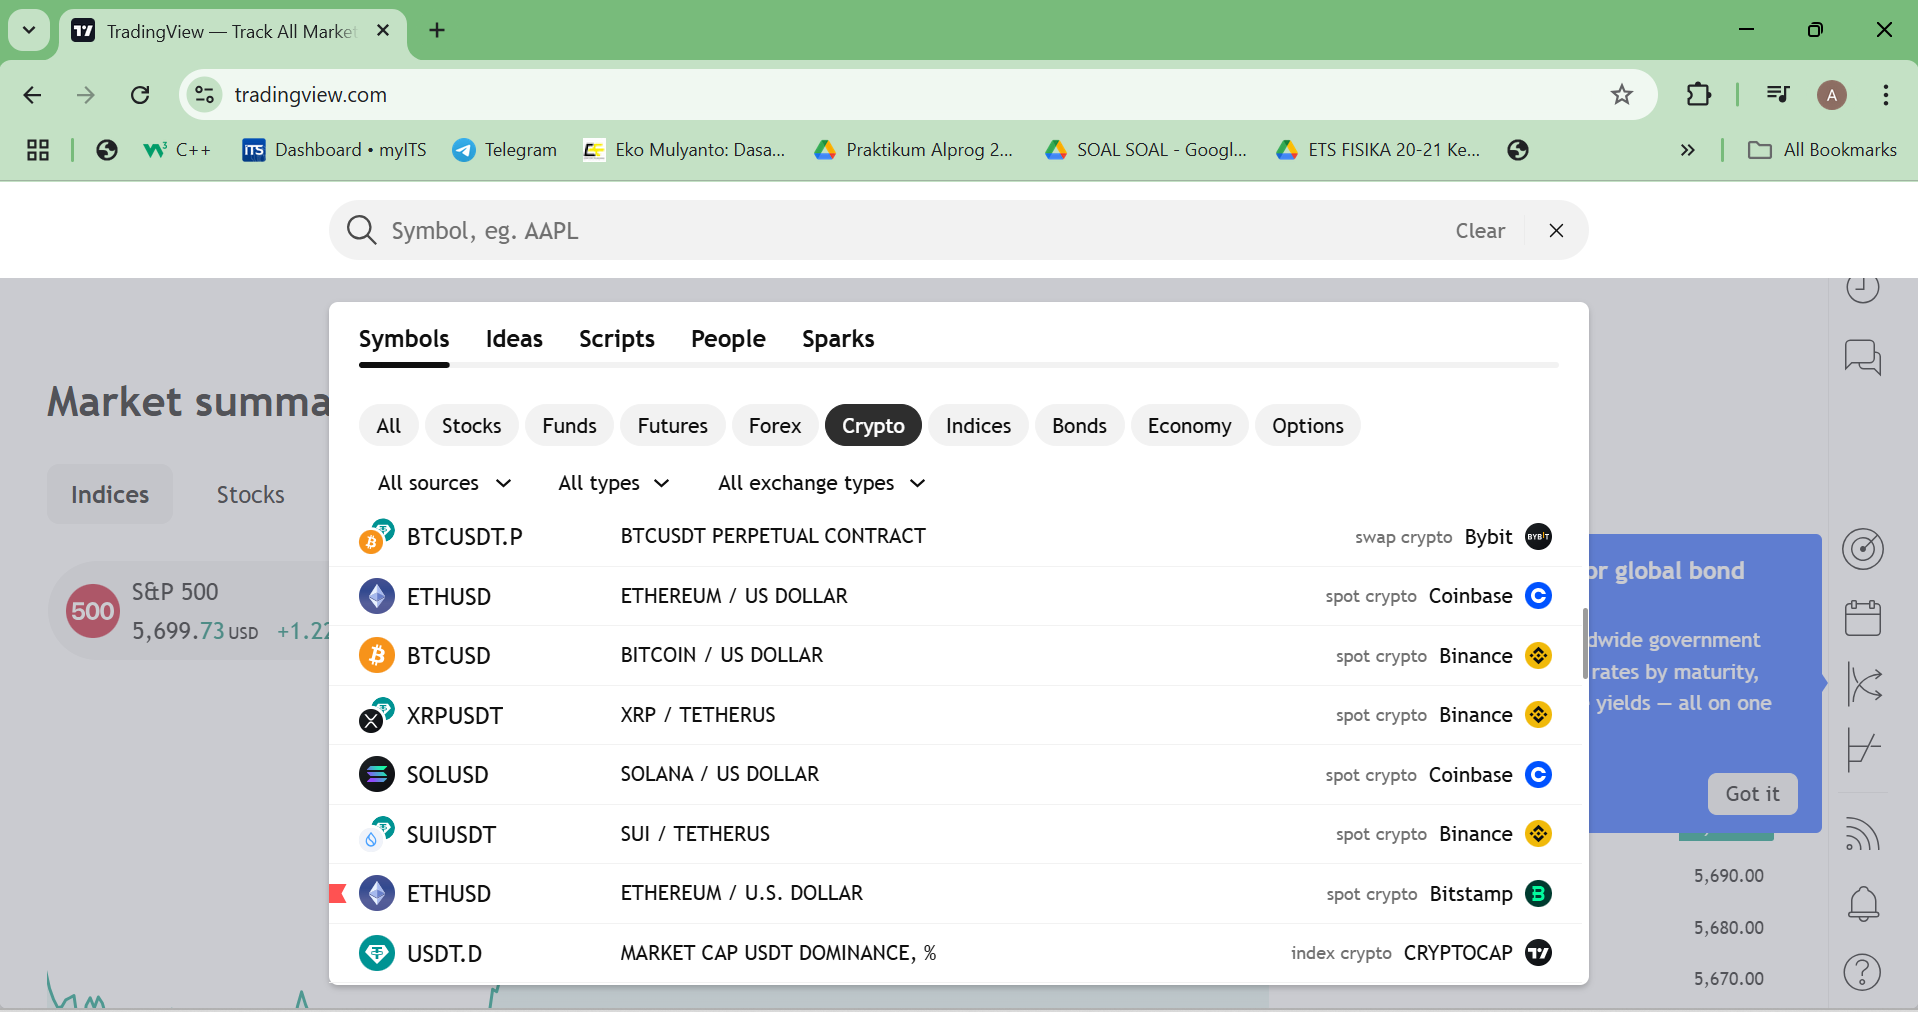
\includegraphics[scale=0.25]{gambar/CRYPTO.png} 
    \caption{Overview Pasar Modal}
    \label{fig:label_gambar}
\end{figure}

\begin{figure} [H] \centering
  % Nama dari file gambar yang diinputkan
  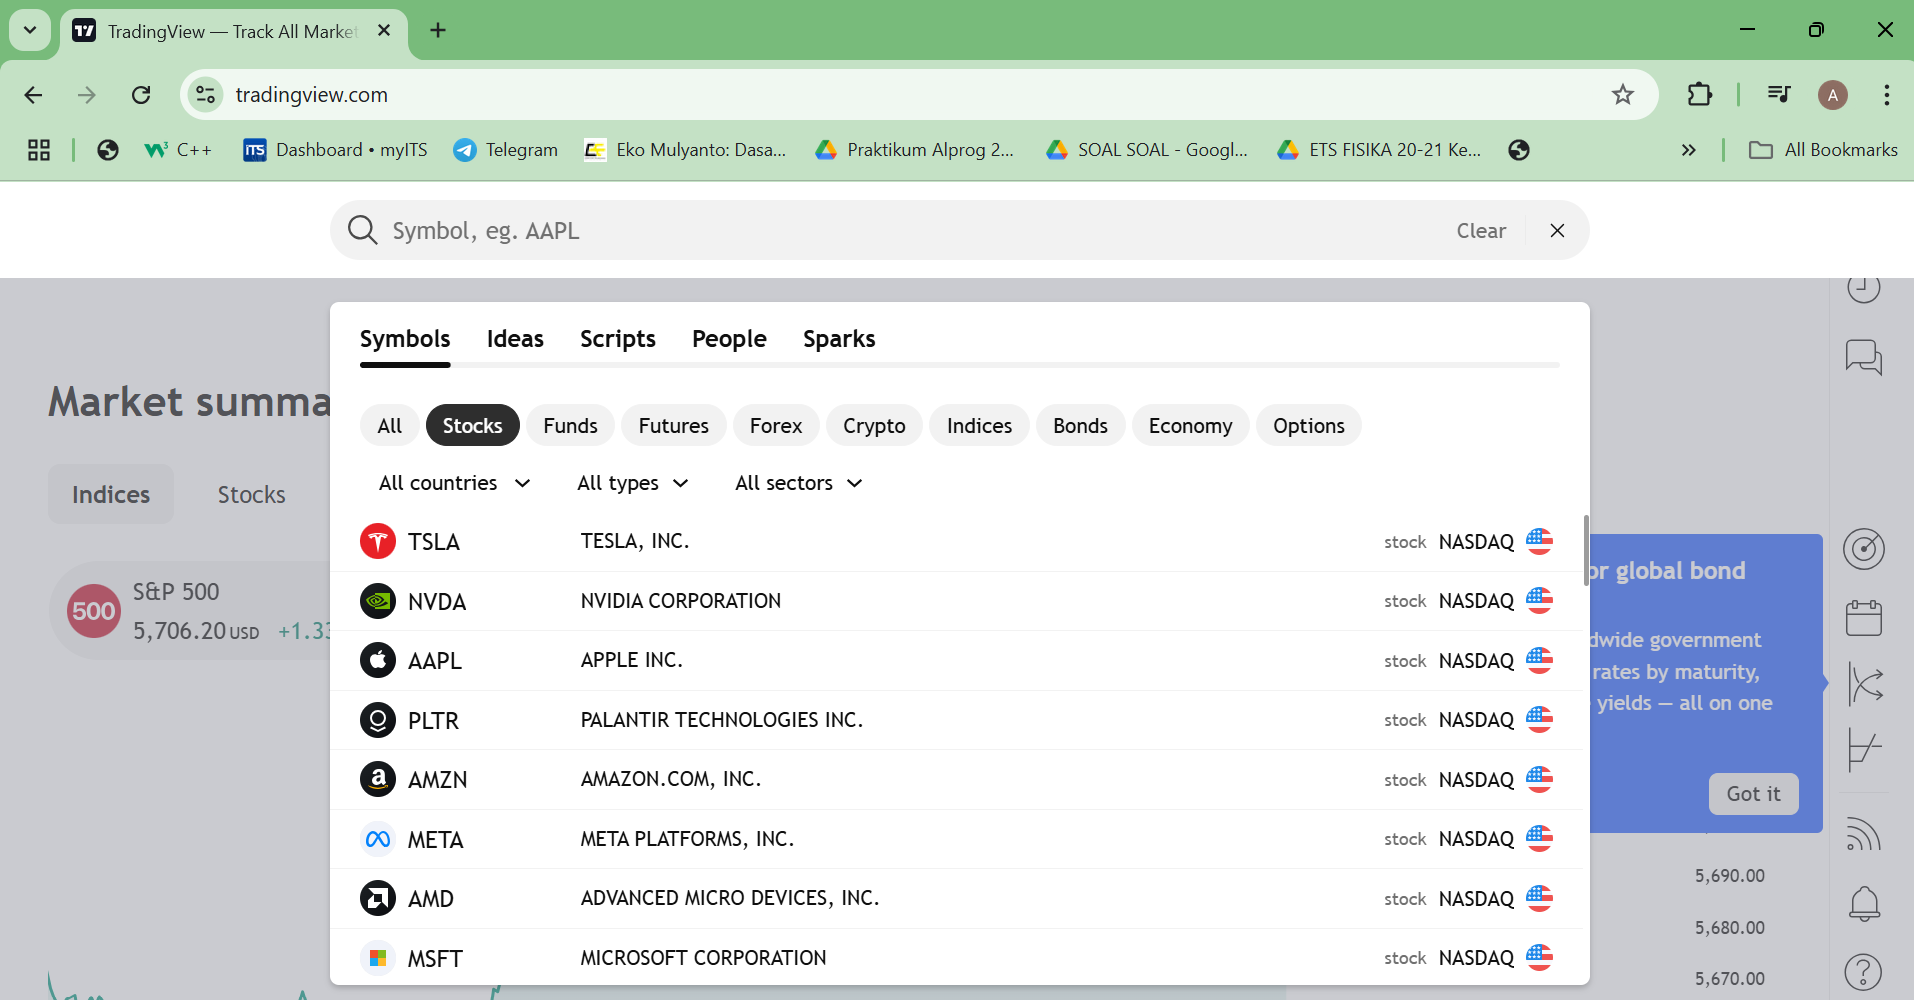
\includegraphics[scale=0.4]{gambar/STOCK.png} 
    \caption{Overview Pasar Modal}
    \label{fig:label_gambar}
\end{figure}
\subsubsection*{2.2.1.1 Pasar Forex}
Pasar Forex, atau pasar valuta asing, adalah pasar global di mana mata uang negara-negara di seluruh dunia diperdagangkan satu sama lain. Ini adalah pasar terbesar dan paling likuid di dunia, dengan volume transaksi harian mencapai lebih dari \$6 triliun pada 2023, menurut Bank for International Settlements (BIS)\autocite{bis2023triennial}. Pasar ini terbuka 24 jam sehari, lima hari seminggu, dan beroperasi tanpa lokasi fisik tunggal\autocite{hull2015options}. Sebagai pasar desentralisasi, forex berlangsung secara elektronik melalui berbagai platform dan sistem perdagangan yang menghubungkan bank, lembaga keuangan, pemerintah, perusahaan besar, dan trader individu.
\begin{enumerate}
    \item Fungsi Pasar Forex
    \begin{itemize}
        \item \textbf{Pertukaran Mata Uang untuk Perdagangan Internasional:} Perusahaan dan negara memerlukan mata uang asing untuk melakukan transaksi internasional. Misalnya, importir dan eksportir perlu membeli atau menjual mata uang asing untuk membayar barang dan jasa.
        \item \textbf{Manajemen Resiko (\textit{Hedging}):} Perusahaan dan investor menggunakan pasar forex untuk melindungi diri dari risiko perubahan nilai tukar yang dapat mempengaruhi pendapatan mereka. Misalnya, sebuah perusahaan yang memiliki eksposur terhadap mata uang asing akan melakukan kontrak derivatif untuk mengurangi potensi kerugian.
        \item \textbf{Spekulasi:}Trader individu dan lembaga keuangan sering berpartisipasi dalam pasar forex untuk meraih keuntungan dengan memprediksi pergerakan harga mata uang. Ini adalah salah satu aktivitas paling populer di pasar forex.
    \end{itemize}
    \item Pasangan Mata Uang (Currency Pairs)
    
    Di pasar forex, mata uang diperdagangkan dalam pasangan. Sebagai contoh, pasangan mata uang seperti EUR/USD (Euro terhadap Dolar AS) atau GBP/JPY (Pound Inggris terhadap Yen Jepang). Setiap pasangan mata uang terdiri dari:
    \begin{itemize}
        \item \textbf{Base Currency (Mata Uang Dasar):} Mata uang pertama dalam pasangan, misalnya Euro (EUR) dalam pasangan EUR/USD.
        \item \textbf{Quote Currency (Mata Uang Kuotasi):} Mata uang kedua dalam pasangan, misalnya Dolar AS (USD) dalam pasangan EUR/USD.
    \end{itemize}
    
    \item Satuan Pergerakan mata uang
    
    Dalam perdagangan forex \textit{(foreign exchange)}, istilah pips atau \textit{"percentage in point"} adalah satuan terkecil perubahan harga mata uang yang diperdagangkan di pasar valuta asing. Pips berfungsi sebagai pengukur pergerakan harga dan menjadi standar bagi para trader untuk menghitung keuntungan dan kerugian dalam transaksi.
    Secara umum, satu pip biasanya setara dengan pergerakan angka desimal keempat dalam pasangan mata uang dengan format empat desimal, misalnya:
    \begin{itemize}
        \item Jika EUR/USD bergerak dari 1.1000 ke 1.1001, maka perubahannya adalah 1 pip.
        \item Untuk pasangan mata uang tertentu seperti USD/JPY, pip dihitung pada angka desimal kedua, misalnya dari 110.00 ke 110.01 berarti 1 pip.
    \end{itemize}
\end{enumerate}
Perdagangan forex dilakukan melalui platform online, dan harga pasangan mata uang dipengaruhi oleh berbagai faktor ekonomi dan politik, termasuk:
Suku bunga, Kebijakan moneter dari bank sentral, tingkat pengangguran, inflasi.Pasar forex sangat volatil dan bisa sangat cepat bergerak. Oleh karena itu, prediksi harga di pasar forex memerlukan teknik analisis yang kuat dan cermat.
\begin{figure} [H] \centering
  % Nama dari file gambar yang diinputkan
  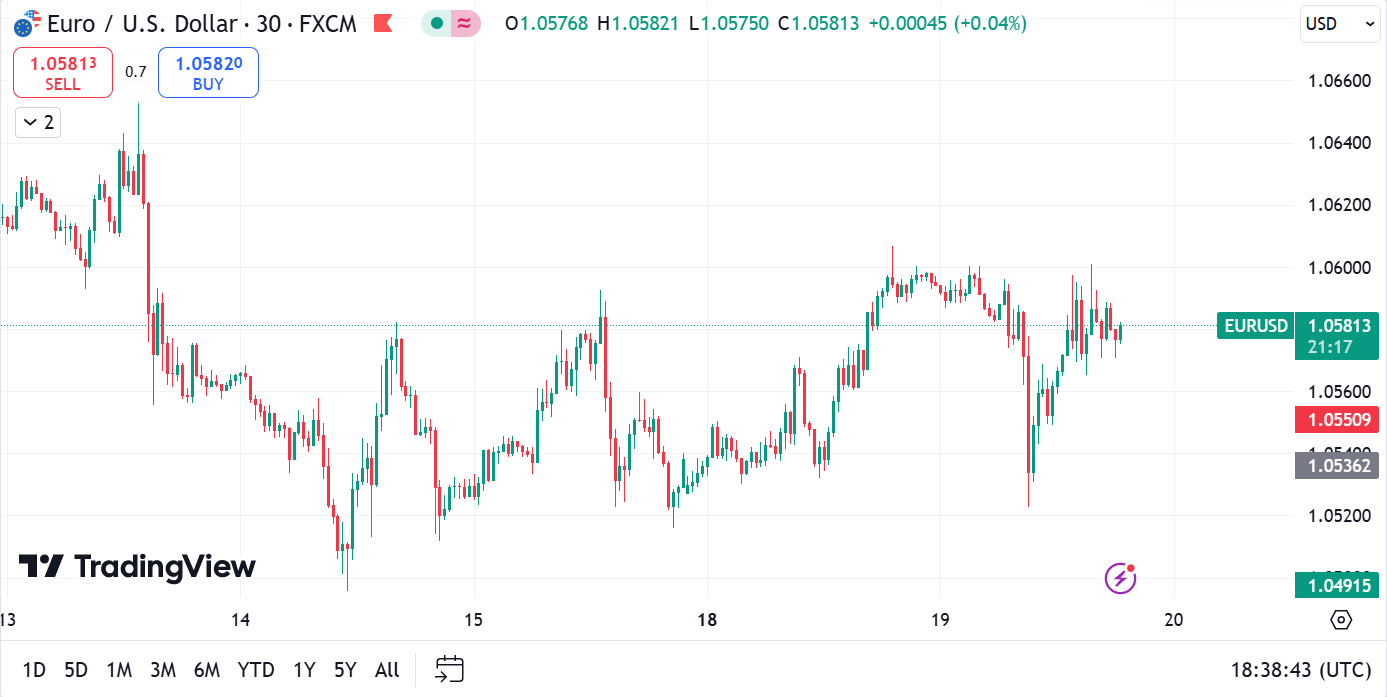
\includegraphics[scale=0.5]{gambar/gambarpasarmodal.png} 
    \caption{Overview forex usd/chf.}
    \label{fig:label_gambar}
\end{figure}

\subsection{Candlestick}
Candlestick adalah salah satu jenis grafik yang digunakan untuk menggambarkan pergerakan harga dalam pasar keuangan, seperti saham, forex, atau komoditas, dalam periode waktu tertentu. Setiap candlestick mewakili informasi tentang harga buka, harga tertinggi, harga terendah, dan harga tutup dalam satu periode waktu tertentu, misalnya per menit, jam, atau hari.

\begin{enumerate}
    \item Struktur Candlestick
    \begin{itemize}
        \item Body (Badan): Bagian tengah candlestick yang menggambarkan perbedaan antara harga buka dan harga tutup pada periode tersebut.
        \item Jika harga tutup lebih tinggi dari harga buka, body candlestick biasanya berwarna hijau atau putih, menandakan tren naik.
        \item Jika harga tutup lebih rendah dari harga buka, body candlestick biasanya berwarna merah atau hitam, menandakan tren turun.
        \item Wick (Sumbu): Garis vertikal yang terletak di atas dan di bawah body, yang menunjukkan harga tertinggi dan terendah dalam periode waktu tersebut.
        \item Upper Wick (Sumbu Atas): Menunjukkan perbedaan antara harga tertinggi dan harga buka (untuk candlestick bullish) atau harga tertinggi dan harga tutup (untuk candlestick bearish).
        \item Lower Wick (Sumbu Bawah): Menunjukkan perbedaan antara harga terendah dan harga buka (untuk candlestick bullish) atau harga terendah dan harga tutup (untuk candlestick bearish).

    \end{itemize}
    \item Elemen Candlestick
    \begin{itemize}
        \item Harga Buka: Harga pada awal periode waktu.
        \item Harga Tutup: Harga pada akhir periode waktu.
        \item Harga Tertinggi: Harga tertinggi yang tercatat selama periode tersebut.
        \item Harga Terendah: Harga terendah yang tercatat selama periode tersebut.
    \end{itemize}
    \item Jenis-Jenis Candlestick
    \begin{itemize}
        \item Bullish Candlestick (Kenaikan Harga): Body candlestick terbentuk dengan harga tutup yang lebih tinggi daripada harga buka, dan umumnya berwarna hijau atau putih. Ini menandakan bahwa harga bergerak naik selama periode tersebut.
        \item Bearish Candlestick (Penurunan Harga): Body candlestick terbentuk dengan harga tutup yang lebih rendah daripada harga buka, dan biasanya berwarna merah atau hitam. Ini menandakan bahwa harga bergerak turun selama periode tersebut.
    \end{itemize}
\end{enumerate}
\begin{figure} [H] \centering
  % Nama dari file gambar yang diinputkan
    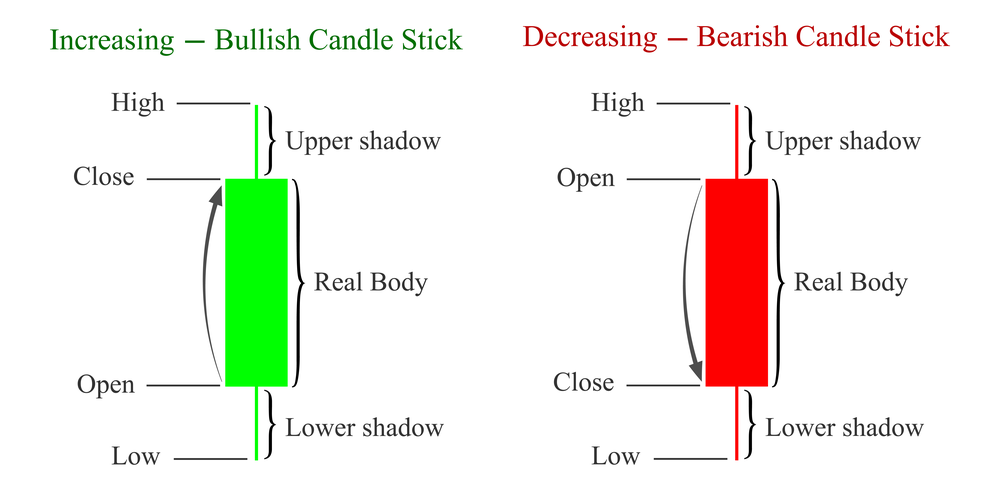
\includegraphics[scale=1.4]{gambar/candlestick.png} 
    \caption{CandleStick}
    \label{fig:label_gambar}
\end{figure}

\subsection{Broker}
Dalam aktivitas perdagangan valuta asing (foreign exchange/forex), broker forex merupakan pihak atau perusahaan yang bertindak sebagai perantara antara trader individu maupun institusi dengan pasar valuta asing global. Pasar forex sendiri merupakan pasar keuangan terbesar di dunia yang bersifat desentralisasi dan beroperasi secara over-the-counter (OTC), sehingga transaksi antar pelaku pasar dilakukan secara langsung melalui jaringan elektronik tanpa adanya bursa terpusat. Dalam hal ini, broker forex menjadi fasilitator yang menyediakan akses bagi trader untuk melakukan transaksi jual beli pasangan mata uang melalui platform trading yang disediakan.

Menurut Babypips (n.d.), broker forex berperan penting karena pasar forex umumnya didominasi oleh institusi keuangan besar, bank sentral, hedge fund, dan perusahaan multinasional. Tanpa adanya broker forex, trader individu tidak memiliki akses langsung ke pasar antar bank tempat transaksi mata uang dalam volume besar dilakukan. Broker forex memberikan berbagai layanan mulai dari penyediaan data harga pasar secara real-time, eksekusi order transaksi, hingga fasilitas manajemen risiko bagi para trader.

Fungsi dan Layanan Broker Forex
Secara umum, fungsi utama broker forex meliputi beberapa hal berikut:
\begin{enumerate}
    \item \textbf{Menyediakan Platform Perdagangan}
    
    Broker forex menyediakan platform trading berbasis desktop maupun mobile, seperti MetaTrader 4 (MT4), MetaTrader 5 (MT5), atau aplikasi berbasis web. Melalui platform ini, trader dapat melakukan analisis harga, eksekusi order, serta pemantauan posisi transaksi secara real-time.
    
    \item \textbf{Memberikan Fasilitas Leverage}

    Broker forex biasanya menawarkan fasilitas leverage, yaitu pinjaman modal dari broker kepada trader agar dapat melakukan transaksi dengan nilai kontrak yang lebih besar dibandingkan dengan modal yang dimiliki. Sebagai contoh, leverage 1:100 memungkinkan trader dengan modal \$100 untuk melakukan transaksi senilai \$10.000. Namun, penggunaan leverage juga meningkatkan potensi risiko kerugian.

    \item \textbf{Menyediakan Harga Pasar dan Spread}

    Broker bertanggung jawab menyediakan harga bid (jual) dan ask (beli) untuk setiap pasangan mata uang. Perbedaan antara harga bid dan ask disebut spread, yang menjadi sumber keuntungan utama bagi broker forex, terutama broker dengan tipe dealing desk.

    \item \textbf{Memberikan Fasilitas Manajemen Risiko}

    Broker forex menyediakan berbagai fitur manajemen risiko seperti \textbf{stop loss, take profit, margin call, dan negative balance protection} untuk membantu trader mengendalikan risiko kerugian dalam aktivitas perdagangan.

    \item \textbf{Penyediaan Edukasi dan Analisis Pasar}

    Banyak broker forex juga menawarkan fasilitas edukasi bagi trader pemula maupun profesional, berupa artikel, video tutorial, webinar, serta analisis pasar harian atau mingguan.

    \item \textbf{Penyediaan Akun Demo}

    Broker forex umumnya menyediakan akun demo yang memungkinkan trader berlatih melakukan transaksi di lingkungan pasar simulasi dengan data harga real-time, tanpa menggunakan dana sungguhan.
\end{enumerate}

Proses kerja broker forex dimulai ketika trader membuka akun trading di broker tertentu, kemudian menyetorkan dana sebagai modal transaksi. Melalui platform trading yang disediakan, trader dapat melakukan analisis pasar dan menempatkan order beli atau jual pasangan mata uang. Broker akan meneruskan order tersebut ke penyedia likuiditas atau pasar antar bank sesuai dengan tipe broker yang digunakan.

Setiap transaksi trader akan dikenakan biaya berupa spread atau komisi sesuai kebijakan broker. Selain itu, broker juga menyediakan fasilitas leverage dan margin yang memungkinkan trader mengendalikan nilai kontrak transaksi dalam jumlah besar, meskipun hanya dengan modal relatif kecil. Broker forex juga bertugas melakukan eksekusi order secara cepat dan akurat agar transaksi dapat terjadi sesuai harga yang diinginkan trader.

Broker forex memiliki peran strategis dalam memastikan kelancaran aktivitas perdagangan valuta asing, khususnya bagi trader individu yang tidak memiliki akses langsung ke pasar antar bank. Selain sebagai perantara transaksi, broker juga berperan sebagai penyedia fasilitas edukasi, informasi pasar, dan teknologi trading. Ketersediaan broker forex yang andal dan teregulasi menjadi faktor penting dalam menciptakan ekosistem perdagangan yang aman, transparan, dan efisien.

\subsection{Analisis Teknikal}
Analisis teknikal adalah metode analisis pasar yang memanfaatkan data historis harga dan volume perdagangan untuk memprediksi pergerakan harga di masa depan. Dalam praktiknya, analisis teknikal lebih menitikberatkan pada pergerakan harga (\textit{price action}) dan pola-pola grafik (\textit{chart patterns}) dibandingkan dengan faktor-faktor fundamental seperti kondisi ekonomi, politik, atau kinerja perusahaan.Analisis teknikal didasarkan pada tiga asumsi utama:

\begin{enumerate}
    \item Harga yang tercatat di pasar sudah mencerminkan semua informasi yang tersedia, baik ekonomi, politik, maupun faktor psikologis.

    \item Pergerakan harga cenderung mengikuti suatu tren, baik itu tren naik (\textit{uptrend}), tren turun (\textit{downtrend}), atau bergerak dalam kisaran tertentu (\textit{sideways}). Prinsip ini menyatakan bahwa tren harga akan berlanjut sampai ada sinyal pembalikan yang jelas.

    \item Pola pergerakan harga cenderung berulang karena faktor psikologi pasar dan perilaku pelaku pasar dari waktu ke waktu. Oleh sebab itu, pola-pola grafik yang muncul di masa lalu dapat digunakan sebagai acuan untuk memprediksi pergerakan harga berikutnya.
\end{enumerate}

Berikut merupakan beberapa teknikal analisis yang biasa digunakan para pelaku pasar modal untuk menganalisis chart pada forex:

\subsubsection*{2.2.4.1 Head \& Shoulders}
Head and Shoulders adalah salah satu pola chart pattern dalam analisis teknikal yang digunakan untuk mengidentifikasi potensi pembalikan arah tren harga di pasar, termasuk dalam pasar forex. Pola ini dianggap sebagai salah satu pola pembalikan (\textit{reversal pattern}) yang paling andal oleh para trader teknikal.

Pola ini dinamakan Head and Shoulders karena bentuknya menyerupai bahu kiri (\textit{left shoulder}), kepala (\textit{head}), dan bahu kanan (\textit{right shoulder}). Secara visual, pola ini terbentuk ketika harga menunjukkan tiga puncak, di mana:

\begin{enumerate}
    \item \textbf{Left Shoulder}: Harga naik ke puncak dan kemudian turun.
    \item \textbf{Head}: Harga kembali naik ke puncak yang lebih tinggi dari puncak sebelumnya, lalu turun lagi.
    \item \textbf{Right Shoulder}: Harga naik lagi, tetapi hanya mencapai puncak yang lebih rendah daripada kepala, lalu turun kembali.
\end{enumerate}

\begin{figure} [H] \centering
  % Nama dari file gambar yang diinputkan
    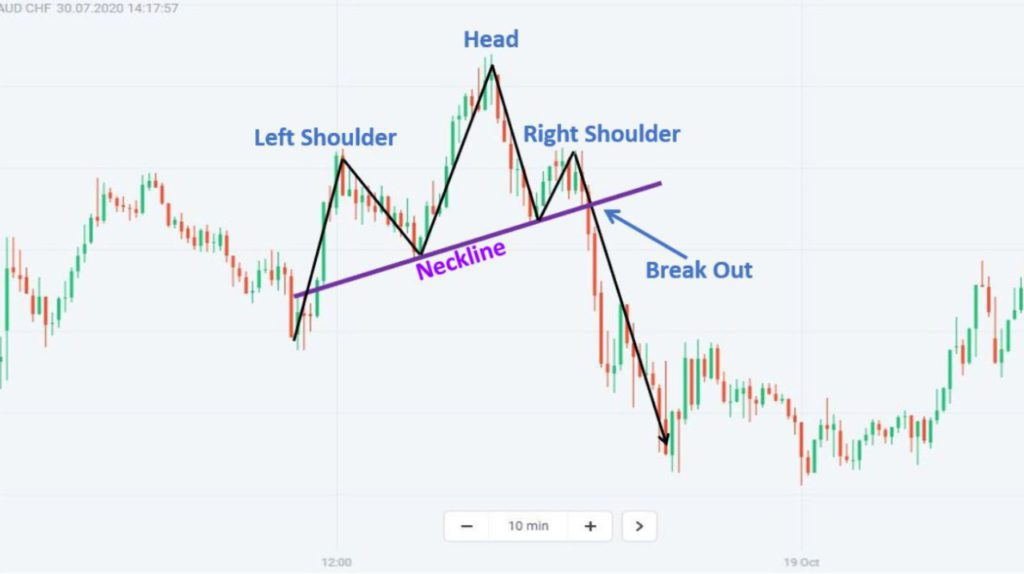
\includegraphics[scale=0.35]{gambar/headshoulders.jpg} 
    \caption{Head \& Shoulders Chart Pattern}
    \label{fig:label_gambar}
\end{figure}

Penurunan setelah bahu kanan biasanya menembus garis leher (\textit{neckline}), yang merupakan garis support yang menghubungkan titik terendah antara head dan kedua shoulders. \textit{Breakout} dari \textit{neckline} ini sering dijadikan sinyal kuat bahwa tren akan berbalik arah.

\subsubsection*{2.2.4.2 Double Top}
Double Top adalah salah satu pola chart pattern dalam analisis teknikal yang menunjukkan potensi pembalikan arah tren (\textit{trend reversal}) dari tren naik menjadi tren turun. Pola ini terbentuk ketika harga mencapai \textit{level resistance} yang sama sebanyak dua kali, namun gagal menembusnya dan kemudian mengalami penurunan.Pola ini banyak digunakan oleh trader forex untuk mengidentifikasi area potensial di mana harga diperkirakan akan mengalami koreksi atau pembalikan tren setelah tren naik.
\begin{figure} [H] \centering
  % Nama dari file gambar yang diinputkan
    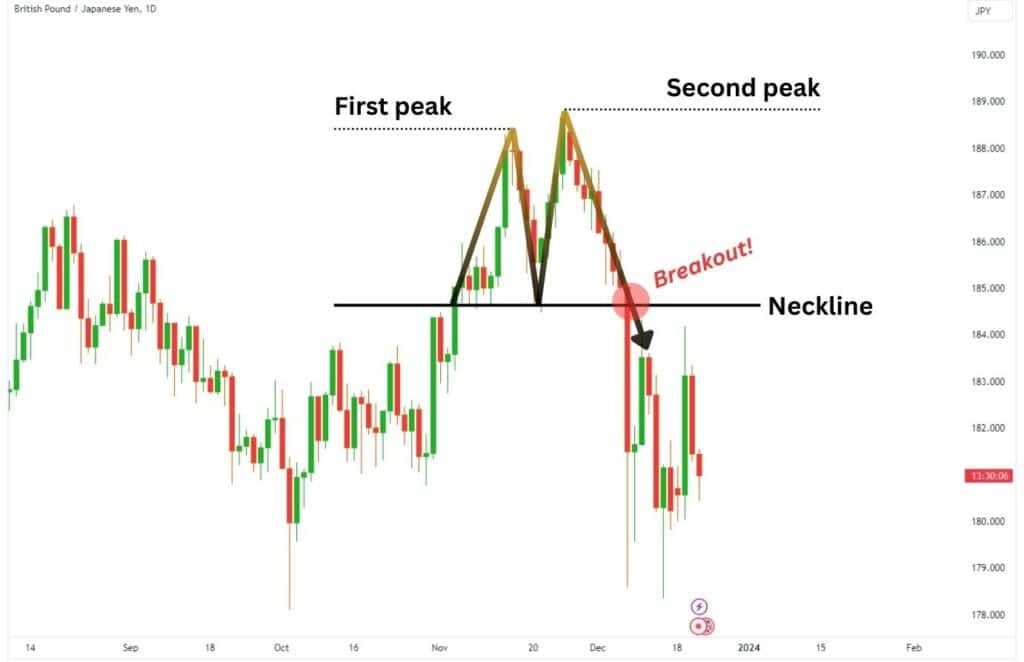
\includegraphics[scale=0.3]{gambar/doubletop.jpg} 
    \caption{Double Top Chart Pattern}
    \label{fig:label_gambar}
\end{figure}

Pola Double Top terdiri dari dua puncak harga (\textit{peak/top}) yang hampir setara ketinggiannya, dipisahkan oleh sebuah lembah (\textit{valley}) di antaranya. Setelah harga membentuk puncak kedua dan gagal menembus puncak pertama, harga biasanya turun ke bawah garis support yang dikenal dengan sebutan \textit{neckline}.

Jika harga berhasil menembus \textit{neckline} ke bawah, maka konfirmasi pola \textit{double top} dianggap valid dan mengindikasikan potensi pembalikan tren dari \textit{bullish} menjadi \textit{bearish}.


\subsection{Deep Learning }
Deep learning adalah cabang dari machine learning yang berfokus pada penggunaan jaringan saraf tiruan (Artificial Neural Networks) dengan banyak lapisan (multi-layered) untuk mempelajari representasi data yang kompleks. Konsep ini terinspirasi dari cara kerja otak manusia yang terdiri dari neuron-neuron yang saling terhubung untuk memproses informasi secara paralel\autocite{lecun2015deep}. Deep learning mulai berkembang pesat seiring dengan kemajuan teknologi komputasi, ketersediaan data dalam jumlah besar , serta peningkatan algoritma optimasi yang efektif. Keunggulan deep learning terletak pada kemampuannya dalam menangkap pola-pola non-linear, mengenali fitur kompleks dari data, serta memproses data dengan dimensi yang tinggi\autocite{goodfellow2016deep}.

Keunggulan utama Transformer terletak pada kemampuan pemrosesan paralel yang signifikan, serta kemampuannya dalam menangkap pola jangka panjang dan dependensi kompleks dalam data\autocite{hochreiter1997long}. Selain itu, positional encoding ditambahkan untuk mempertahankan informasi urutan waktu pada data time series. Dalam prediksi harga pasar modal, arsitektur Time Series Transformer memanfaatkan kemampuan self-attention untuk menganalisis fluktuasi historis harga seperti Open, High, Low, dan Close (OHLC). Hal ini memungkinkan model mempelajari pola volatilitas pasar secara lebih akurat dan efisien. Dengan fleksibilitas input serta kemampuannya dalam memproses data berukuran besar, Time Series Transformer menjadi solusi yang efektif dalam meningkatkan akurasi prediksi pada data pasar modal.

\subsection{Deret Waktu \textit{(Time Series)}}
Deret waktu atau time series adalah serangkaian data yang dikumpulkan atau diukur secara berurutan berdasarkan waktu. Data ini memiliki karakteristik penting yaitu dependensi temporal, di mana nilai pada waktu tertentu bergantung pada nilai-nilai sebelumnya atau masa lalu. Analisis deret waktu bertujuan untuk memahami pola historis dari data dan melakukan prediksi terhadap nilai di masa depan\autocite{box2015time}. Deret waktu sering digunakan dalam berbagai bidang seperti ekonomi, keuangan, cuaca, dan industri untuk memprediksi tren dan fluktuasi. Dalam konteks pasar modal, data deret waktu terdiri dari informasi historis seperti harga Open, High, Low, dan Close (OHLC) yang memiliki sifat dinamis dan volatil, serta sangat dipengaruhi oleh faktor internal maupun eksternal.

Metode tradisional seperti MA (Moving Average) telah lama digunakan untuk analisis deret waktu karena kemampuannya menangkap pola linear dalam data. Namun, metode ini memiliki keterbatasan dalam memodelkan pola yang non-linear dan kompleks, serta kesulitan dalam menangkap dependensi jangka panjang. Kelemahan ini mendorong penggunaan metode berbasis deep learning seperti Recurrent Neural Networks (RNN) dan Long Short-Term Memory (LSTM), yang dirancang khusus untuk menangani data sekuensial. LSTM memperbaiki kelemahan RNN dengan mekanisme gates yang memungkinkan model menangkap hubungan temporal jangka pendek maupun jangka panjang secara lebih efektif. Meski begitu, LSTM masih memiliki tantangan dalam efisiensi komputasi karena proses pelatihan yang bersifat berurutan (sequential).

Untuk mengatasi keterbatasan tersebut, arsitektur Transformer dikembangkan sebagai solusi yang lebih efisien dan akurat dalam analisis deret waktu. Berbeda dengan RNN dan LSTM, Transformer menggunakan self-attention mechanism untuk mempelajari hubungan temporal di seluruh titik waktu secara paralel, sehingga memungkinkan pemrosesan yang lebih cepat dan efektif. Dengan positional encoding, Transformer tetap dapat mempertahankan informasi urutan waktu dalam data time series. Pada prediksi harga pasar modal, pendekatan ini memungkinkan model untuk menangkap pola fluktuasi harga dengan lebih baik, termasuk interaksi kompleks antar variabel seperti harga Open, High, Low, dan Close. Dengan demikian, penggunaan Time Series Transformer menjadi pendekatan yang unggul dalam analisis dan prediksi deret waktu karena mampu memodelkan dependensi temporal jangka panjang, menangani non-linearitas data, serta meningkatkan efisiensi komputasi dalam proses pelatihan. 

Dalam prediksi harga pasar modal, data deret waktu sering digunakan untuk menangkap pola musiman, siklus, atau tren jangka panjang.Komponen utama deret waktu adalah
\begin{enumerate}
    \item Trend: Komponen deret waktu yang menggambarkan pola perubahan jangka panjang dalam data. Trend menunjukkan arah umum pergerakan data, apakah naik, turun, atau tetap stabil selama periode waktu tertentu. Misalnya, jika penjualan suatu produk terus meningkat selama beberapa tahun, maka ada trend naik pada data penjualan tersebut.
    \begin{figure} [H] \centering
    % Nama dari file gambar yang diinputkan
    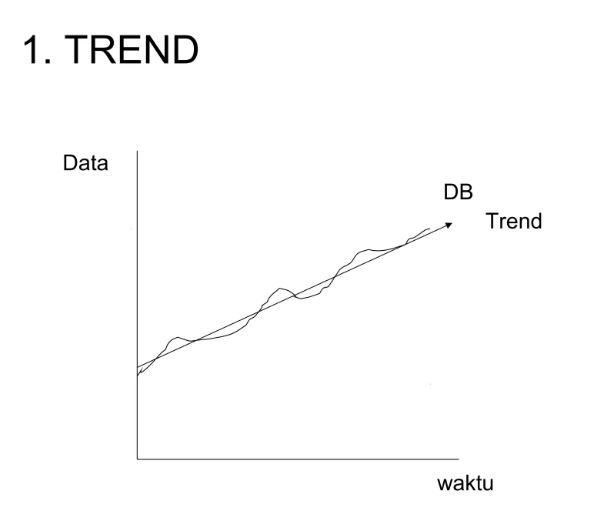
\includegraphics[scale=0.8]{gambar/deret waktu trend.png} 
    \caption{Pola Trend}
    \label{fig:label_gambar}
    \end{figure}
    \item Musiman (Seasonality): Fluktuasi teratur dalam data yang terjadi pada interval waktu tertentu, biasanya dalam siklus yang berulang secara tahunan, bulanan, atau mingguan. Komponen musiman mencerminkan pola yang terjadi pada waktu tertentu dalam setahun atau bulan tertentu.Pola berulang berdasarkan waktu, seperti kuartal atau tahun.
    \begin{figure} [H] \centering
     % Nama dari file gambar yang diinputkan
    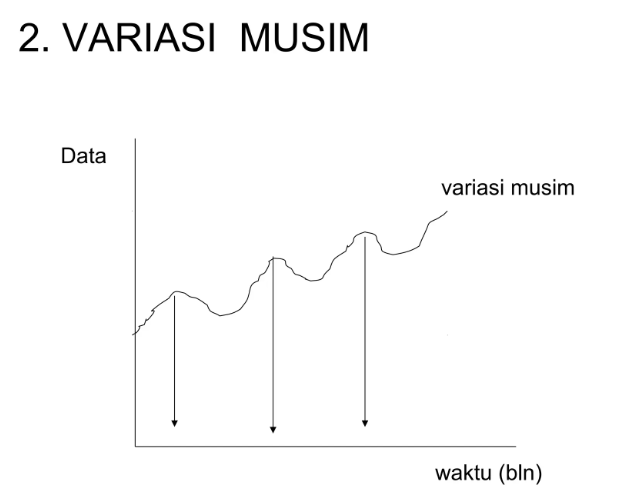
\includegraphics[scale=0.8]{gambar/deret waktu musiman.png} 
    \caption{Pola Musiman.}
    \label{fig:label_gambar}
    \end{figure}
    \item Noise: Noise merujuk pada fluktuasi atau gangguan acak dalam data yang tidak dapat dijelaskan oleh komponen trend atau musiman. Noise adalah variabilitas yang tidak teratur dan tidak dapat diprediksi dalam data. Ini sering kali disebabkan oleh faktor eksternal yang tidak terkontrol, kesalahan pengukuran, atau faktor lain yang tidak terkait dengan pola jangka panjang atau musiman. Noise sering dianggap sebagai "gangguan" dalam analisis deret waktu, karena sulit untuk diprediksi atau dimodelkan secara langsung.
    \begin{figure} [H] \centering
     % Nama dari file gambar yang diinputkan
    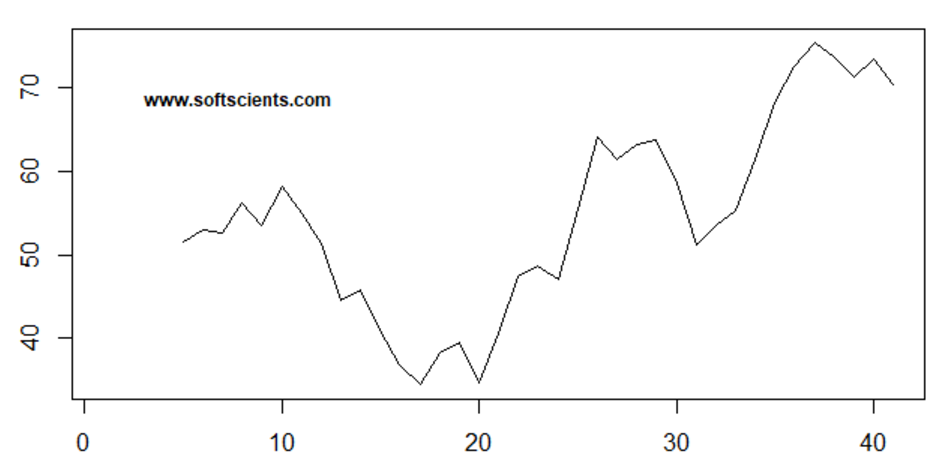
\includegraphics[scale=0.8]{gambar/deret waktu noise.png} 
    \caption{Pola Noise.}
    \label{fig:label_gambar}
\end{figure}
\end{enumerate}

\subsection{Time Series Transformer \textit{(TST)}}
Time Series Transformer adalah model deep learning yang dikembangkan berdasarkan arsitektur Transformer yang pertama kali diperkenalkan oleh Vaswani et al. (2017) dalam paper "Attention Is All You Need". Transformer dirancang untuk menangani data sekuensial dengan pendekatan self-attention mechanism, yang memungkinkan model untuk mempelajari hubungan antara elemen dalam urutan data secara paralel dan efisien. Berbeda dengan metode tradisional seperti ARIMA atau model berbasis Recurrent Neural Networks (RNN) dan Long Short-Term Memory (LSTM), Transformer tidak memproses data secara sequential melainkan menggunakan mekanisme perhatian untuk mengidentifikasi dependensi jangka pendek maupun jangka panjang dalam data\autocite{hochreiter1997long}. Hal ini membuat Transformer unggul dalam menangani long-term dependencies dan non-linear relationships yang sering muncul pada data time series, termasuk prediksi harga pasar modal.

Pada model Time Series Transformer, komponen self-attention memainkan peran utama dalam mengidentifikasi kontribusi dari setiap titik waktu terhadap prediksi masa depan. Mekanisme ini bekerja dengan menghitung bobot perhatian antara setiap titik waktu dalam data input, di mana nilai perhatian yang lebih besar diberikan pada titik-titik yang dianggap lebih relevan\autocite{vaswani2017attention}. Untuk mempertahankan informasi urutan waktu, Time Series Transformer menggunakan positional encoding, yang menambahkan informasi posisi ke dalam representasi data sebelum diolah oleh model. Dengan ini, model dapat memahami konteks temporal dari data time series meskipun pemrosesan dilakukan secara paralel.

Dalam konteks prediksi harga pasar modal, Time Series Transformer digunakan untuk menganalisis data historis seperti harga Open, High, Low, dan Close (OHLC). Kemampuan model ini untuk mempelajari pola volatilitas yang kompleks serta menangkap hubungan temporal antar variabel memungkinkan prediksi yang lebih akurat dibandingkan metode konvensional\autocite{goodfellow2016deep}. Selain itu, fleksibilitas arsitektur Transformer memudahkan integrasi dengan berbagai fitur tambahan, seperti indikator teknikal atau data ekonomi makro, yang sering digunakan dalam analisis pasar. Dengan efisiensi komputasi dan performa yang unggul dalam menangkap pola kompleks, Time Series Transformer menjadi pendekatan yang sangat cocok untuk prediksi harga pasar modal dalam skenario data berskala besar.



Komponen Utama Time Series Transformer
\begin{enumerate}
    \item Attention Mechanism:
    \begin{itemize}
        \item Mengidentifikasi hubungan antara titik-titik data deret waktu secara global, sehingga mampu menangkap pola jangka panjang dan interaksi antarvariabel.
        \item Dua varian populer: Self-Attention dan Multi-Head Attention.
    \end{itemize}
    \item Positional Encoding:
    \begin{itemize}
        \item Karena Transformer tidak memiliki pemahaman urutan data bawaan, informasi posisi ditambahkan untuk menjaga konteks urutan waktu.
    \end{itemize}
    \item Encoder-Decoder Architecture:
     \begin{itemize}
        \item Encoder: Memahami pola historis dari data input.
        \item Decoder: Menghasilkan prediksi untuk langkah waktu berikutnya.
    \end{itemize}
    
\end{enumerate}
% Contoh penggunaan referensi dari persamaan
Time Series Transformer mempunyai arsitektur sebagai berikut.
\begin{figure} [H] \centering
  % Nama dari file gambar yang diinputkan
  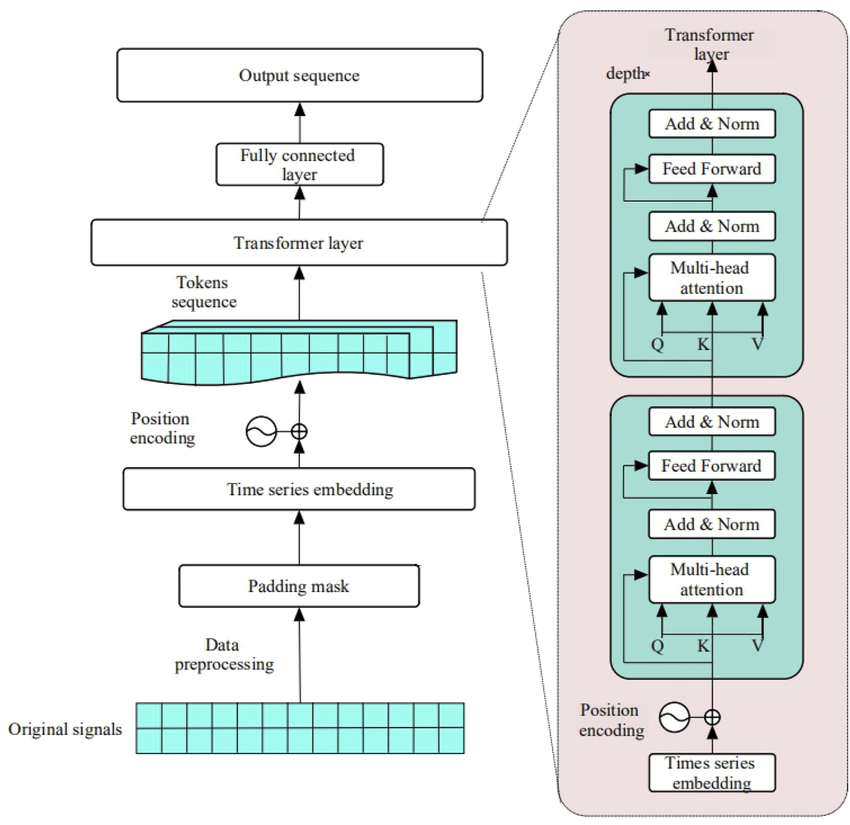
\includegraphics[scale=1.2]{gambar/gambar TST.png} 
    \caption{Arsitektur Time Series Transformer.}
    \label{fig:label_gambar}
\end{figure}
\begin{enumerate}
    \item \textbf{Data Prepocessing \& Embedding:} dalam lapisan ini terdapat beberapa langkah yang akan dilakukan. Data akan dinormalisasikan dengan cara membagi data menjadi skala yang lebih kecil menggunakan min-max scalling, dan padding digunakan untuk memastikan bahwa semua input memiliki panjang yang sama untuk membantu model memahami perbedaan antar fitur.Setelah itu akan ditambahkan keterangan waktu seperti menit jam atau hari untuk membantu model menangkap pola dari data. menginput dataset deret waktu multivarian dan memberikan input urutan waktu yang benar.
    \item \textbf{Transformer layer:} Lapisan ini akan memulai untuk mengolah data yang telah disiapkan di tahap selanjutnya,inti dari transformer adalah \textit{Self-attention} yang memungkinkan model untuk memahami hubungan antar eleman di dalam data.Layer ini akan mempelajari dan  menangkap hubungan temporal time series dari data, dan juga menggunakan beberapa kepala\textit{(heads)} untuk menangkap berbagai jenis hubungan temporal dalam data.Berikut adalah formula yang dipakai untuk \textit{Multi-Head Attention}
   \item \textbf{Output layer:} Lapisan output dalam Time Series Transformer bertugas untuk mengubah representasi terakhir dari encoder dan decoder untuk menjadi prediksi yang sesuai dari dataset yang telah diberikan. Lapisan ini sangat penting karena menentukan bagaimana model mengolah dan mempelajari informasi yang telah diberikan dan mengeluarkan hasil yang dapat digunakan.

\end{enumerate}
